\begin{frame}
	\frametitle{Bandas críticas de energia}
		\only<1>{
			\framesubtitle{Definições}
			\par Definem os intervalos em que serão calculadas as energias.\newline
			\begin{columns}
				\column{0.5\textwidth}
					\par A energia de um sinal digital $s[\cdot]$ com $M$ amostras é definida como
					\begin{equation}
						E = \sum\limits_{i=0}^{M-1}(s_i)^2 \qquad.   
					\end{equation}
				\column{0.5\textwidth}
					\begin{itemize}
						\item \textbf{BARK:} 20, 100, 200, 300, 400, 510, 630, 770, 920, 1080, 1270, 1480, 1720, 2000, 2320, 2700, 3150, 3700, 4400, 5300, 6400, 7700, 9500, 12000, 15500.
						\item \textbf{MEL:} 20, 160, 394, 670, 1000, 1420, 1900, 2450, 3120, 4000, 5100, 6600, 9000, 14000.
					\end{itemize}
			\end{columns}
		}
		\only<2>{
			\framesubtitle{Cálculo de vetores de características com BARK}
			\begin{figure}
				\centering
				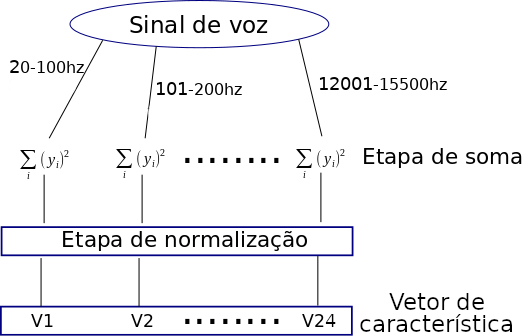
\includegraphics[width=0.7\linewidth]{../monography/images/barkFeatureVect}
			\end{figure}
		}
		\only<3>{
			\framesubtitle{Cálculo de vetores de características com MEL}
			\begin{figure}
				\centering
				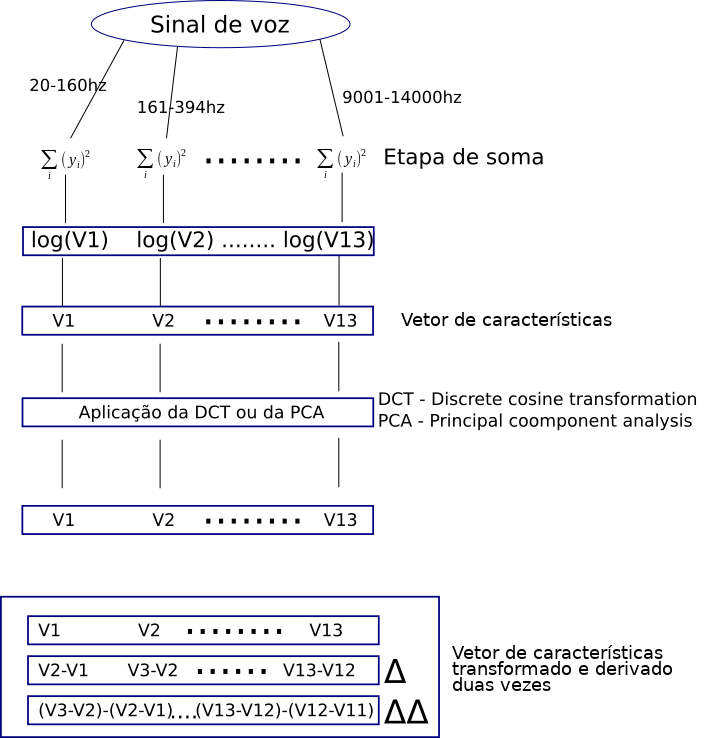
\includegraphics[width=0.5\linewidth]{../monography/images/melFeatureVect}
			\end{figure}
		}
\end{frame}